\documentclass[aspectratio=169]{beamer}
%% Choose aspect ratio and other standard options:
[aspectratio=169] % 16:9 (default)
% [aspectratio=43]  % 4:3 

\hypersetup{pdfpagemode=FullScreen}

\usetheme[standard]{tugraz2018}
%% Choose main theme variant:
% [standard]        % standard (default)
% [institute]       % with institute's graphical acronym on the left
% [minimal]         % with reduced visuals

%% Choose your font style:
%                   % Helvetica (default for Corporate Design)
% [webfont]         % Source Sans Pro (as used on tugraz.at)
% [nofont]          % no font loaded - Computer Modern Sans

%% For more options, see README.pdf

\usepackage[utf8]{inputenc}
\usepackage[english]{babel}
%% Choose your main language:
% [ngerman]   % German
[english]   % English


%% Add your own packages, macros, etc.
\usepackage[absolute,overlay]{textpos}
% ...


%% Enter presentation metadata
\title[AndroGUARD]{AndroGUARD:\\Mitigation of Sensor Fingerprinting\\on Android}
\author{Gergö Kranz}
\date{20.02.2025}
\institute{ISEC}
\instituteurl{www.isec.tugraz.at}

%% Logos
% \institutelogo{beamerthemetugraz/institute/kurz}  % graphical acronym for [institute] theme (left margin)
% \additionallogo{figures/logo}  % additional institute/department logo (footline; optional)
% \logobar{Supported by: ...}  % sponsors (titlepage; optional)


\begin{document}

\begin{frame}[plain]
  \maketitle
\end{frame}


\begin{frame}{Outline}
  \begin{minipage}{0.49\textwidth} 
    \tableofcontents
  \end{minipage}
  \hfill
  \begin{minipage}{0.49\textwidth} 
    \begin{figure}
      \centering
      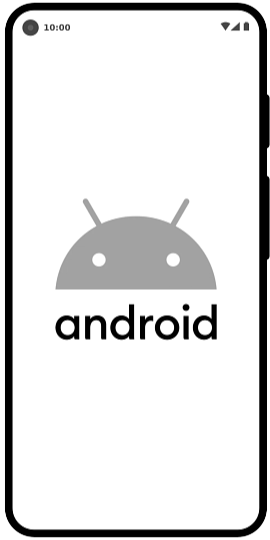
\includegraphics[height=0.5\textheight]{figures/android_device.png}
    \end{figure}
  \end{minipage}
\end{frame}


\section{Introduction}

\begin{frame}{Introduction}
  \begin{minipage}{0.49\textwidth} 
    \begin{itemize}
      \item Misuse of the Android API
      \pause
      \item Used for targeted advertisements
      \pause
      \item Does not require user permission
    \end{itemize}
  \end{minipage}
  \hfill
  \begin{minipage}{0.49\textwidth} 
    \begin{figure}
      \centering
      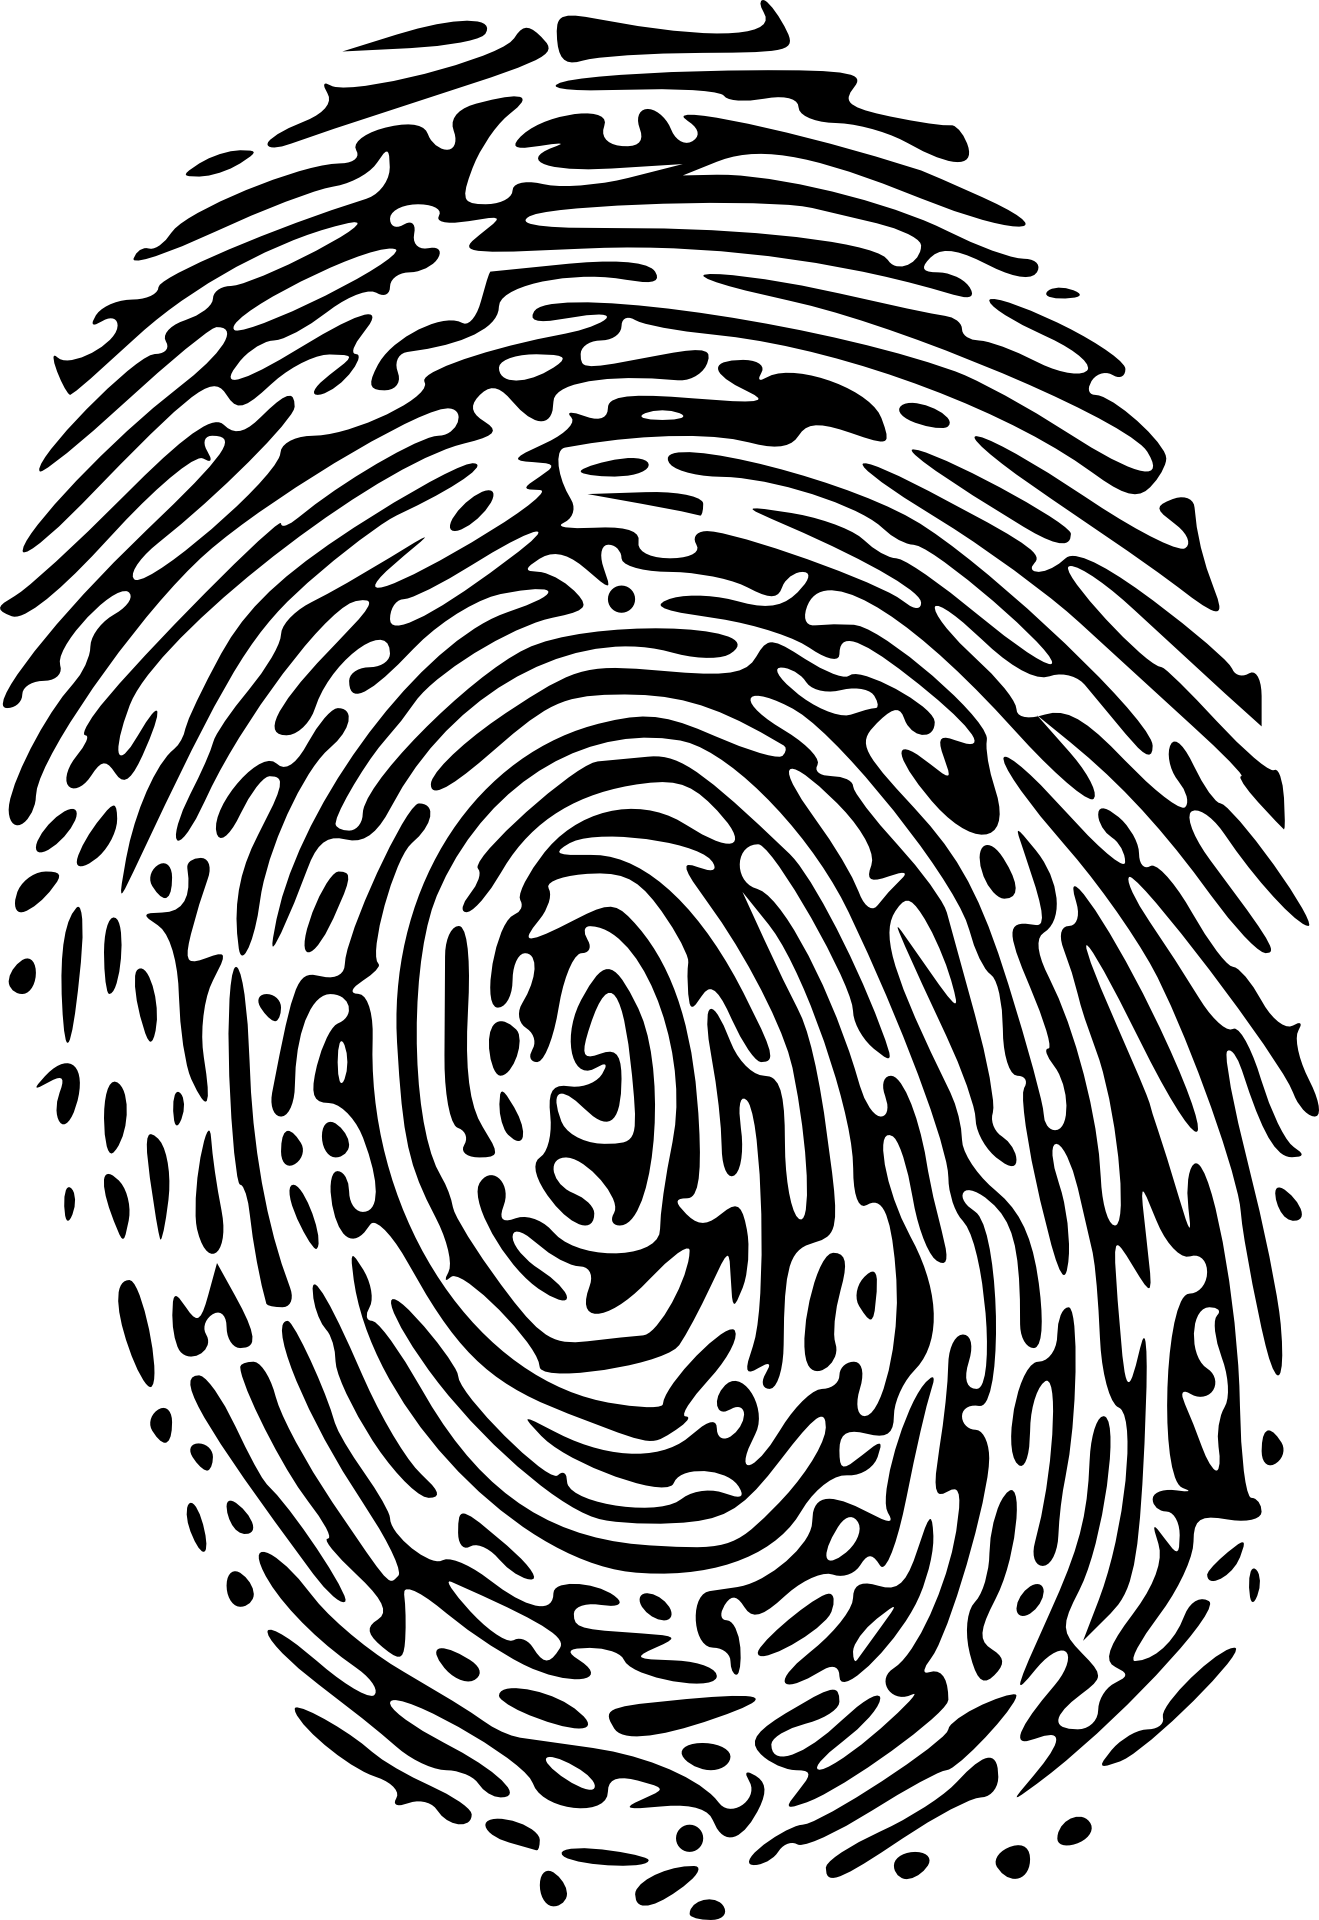
\includegraphics[height=0.5\textheight]{figures/fingerprint.png}
    \end{figure}
  \end{minipage}
\end{frame}


\section{Background}

\begin{frame}{Smartphone Fingerprinting}
  \begin{minipage}{0.49\textwidth} 
    \begin{itemize}
      \item Similar to browser fingerprinting
      \pause
      \item Not as known as browser fingerprinting
      \pause
      \item Zero permission identifiers
      \pause
      \item Personalized configurations
    \end{itemize}
  \end{minipage}
  \hfill
  \begin{minipage}{0.49\textwidth} 
    \begin{figure}
      \centering
      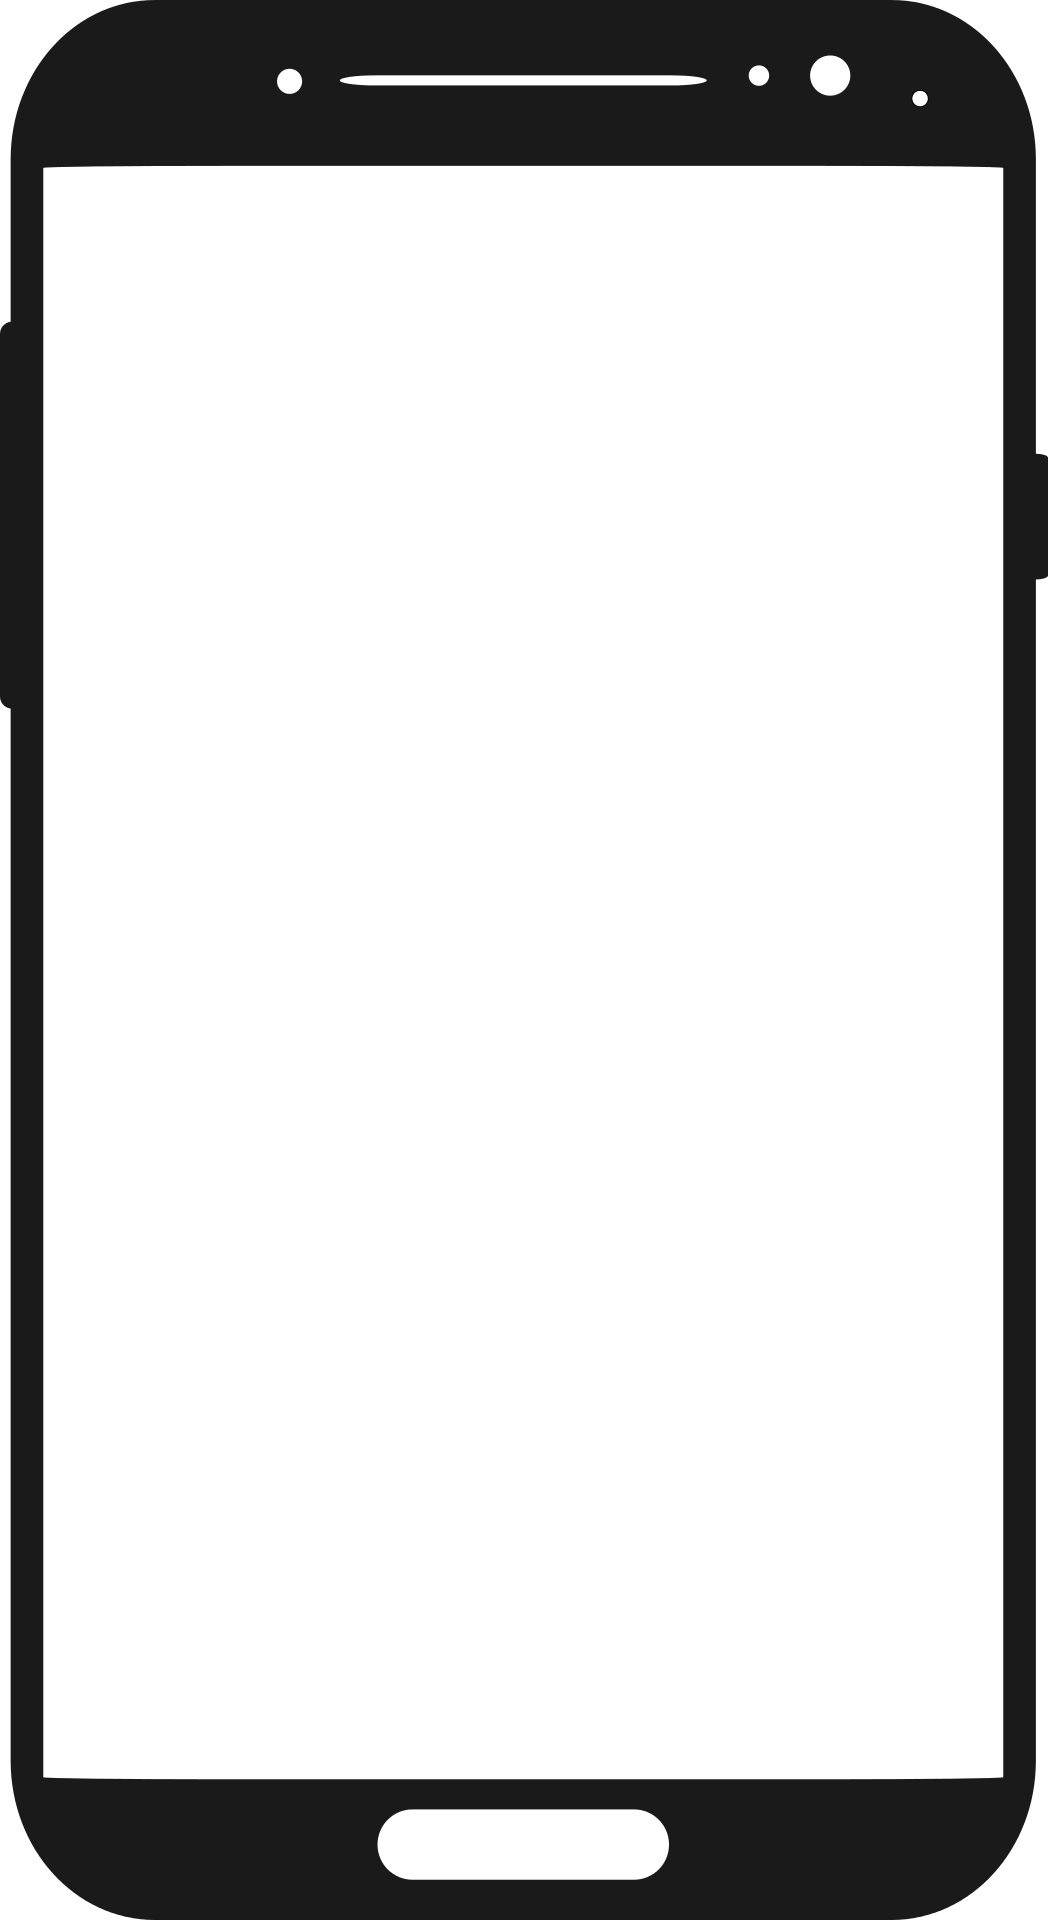
\includegraphics[height=0.5\textheight]{figures/smartphone.png}
    \end{figure}
  \end{minipage}
\end{frame}


\section{Sensor Fingerprinting}

\begin{frame}{Fingerprinting Sensors}
  \begin{minipage}{0.49\textwidth} 
    \begin{itemize}
      \item Measurement inaccuracy of sensors
      \pause
      \item Simple to fingerprint via machine learning algorithmus
      \pause
      \item Constant over the sensors lifetime
    \end{itemize}
  \end{minipage}
  \hfill
  \begin{minipage}{0.49\textwidth}
    \begin{figure}
      \centering
      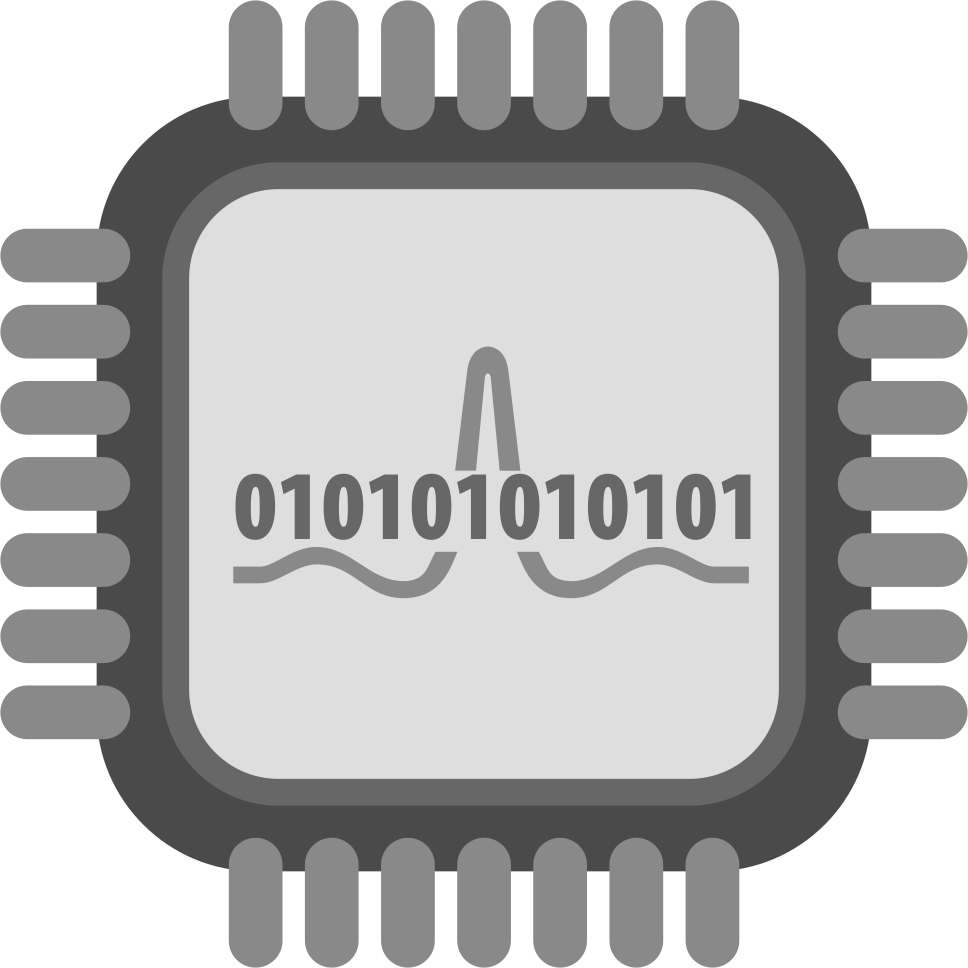
\includegraphics[height=0.5\textheight]{figures/analog.png}
    \end{figure}
  \end{minipage}
\end{frame}


\section{Methodology}

\begin{frame}{Main Question}
  \begin{minipage}{0.65\textwidth} 
    How to protect against sensor fingerprinting
  \end{minipage}
  \hfill
  \begin{minipage}{0.34\textwidth} 
    \begin{figure}
      \centering
      
\includegraphics[height=0.5\textheight]{figures/question.png}
    \end{figure}
  \end{minipage}
\end{frame}

\begin{frame}{Proposed Solutions}
  \begin{minipage}{0.49\textwidth} 
    Calibration
    \begin{itemize}
      \item Systematic adjustment of sensor readings
      \item Correcting the sensor data
    \end{itemize}
  \end{minipage}
  \hfill
  \begin{minipage}{0.49\textwidth} 
    Noise Generation
    \begin{itemize}
      \item Introduces variability into the sensor data
      \item Masks the original values
    \end{itemize}
  \end{minipage}
\end{frame}

\begin{frame}{Challenges}
  \begin{minipage}{0.49\textwidth} 
    Calibration
    \begin{itemize}
      \item Requires user awareness\\and interaction
      \item Requires precision
    \end{itemize}
  \end{minipage}
  \hfill
  \begin{minipage}{0.49\textwidth} 
    Noise Generation
    \begin{itemize}
      \item Degrade the functionality of applications
      \item Code has to be modified
    \end{itemize}
  \end{minipage}
\end{frame}


\section{Approach}

\begin{frame}{Our Methodology}
  \begin{minipage}{0.49\textwidth} 
    \begin{itemize}
      \item Noise Generation
      \item Patch application vie A2P2 framework
    \end{itemize}
  \end{minipage}
  \hfill
  \begin{minipage}{0.49\textwidth} 
    \begin{figure}
      \centering
      
\includegraphics[height=0.5\textheight]{figures/android.png}
    \end{figure}
  \end{minipage}
\end{frame}

\begin{frame}{Modifying the Sensor API}
  \begin{minipage}{0.49\textwidth} 
    \begin{itemize}
      \item Intercept calls to registerListener method
      \item Provide modified values to onSensorChanged method
    \end{itemize}
  \end{minipage}
  \hfill
  \begin{minipage}{0.49\textwidth} 
    \begin{figure}
      \centering
      
\includegraphics[height=0.5\textheight]{figures/code.png}
    \end{figure}
  \end{minipage}
\end{frame}

\begin{frame}{Noise Generation}
  \begin{minipage}{0.49\textwidth} 
    \begin{itemize}
      \item Adds random gain and offset to every value
      \item Masks values
      \item Loss of precision
    \end{itemize}
  \end{minipage}
  \hfill
  \begin{minipage}{0.49\textwidth} 
    \begin{figure}
      \centering
      
\includegraphics[height=0.5\textheight]{figures/noise.png}
    \end{figure}
  \end{minipage}
\end{frame}


\section{Implementation}

\begin{frame}<1>[label=impl]{Implementation}
  \begin{minipage}{0.49\textwidth} 
    \begin{itemize}
      \item Intercept Method
      \pause
      \item Noise Generating Function
      \pause
      \item Random Value Generation Function
    \end{itemize}
  \end{minipage}
  \hfill
  \begin{minipage}{0.49\textwidth} 
    \begin{figure}
      \centering
      
\includegraphics[height=0.5\textheight]{figures/java.png}
    \end{figure}
  \end{minipage}
\end{frame}

\begin{frame}{Intercept Method}
  \begin{textblock*}{\textwidth}(30pt,50pt)
  \begin{figure}
    \centering
    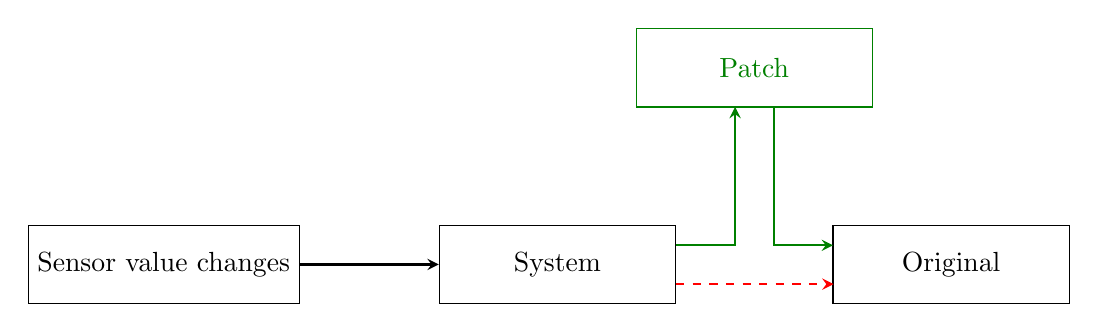
\begin{tikzpicture}
      \tikzstyle{process} = [rectangle, minimum width=3cm, minimum height=1cm, text centered, draw=black]

      \node (sensor) [process] at (0,0) {Sensor value changes};
      \node (system) [process] at (5,0) {System};
      \node (patch) [process, black!50!green] at (7.5,2.5) {Patch};
      \node (function) [process] at (10,0) {Original};

      \draw [thick, ->, >=stealth] (sensor) -- (system);
      \draw [thick, ->, >=stealth, red, dashed] (system.east)+(0,-0.25) -- +(2,-0.25);
      \draw [thick, ->, >=stealth, black!50!green] (system.east)+(0,0.25) -| +(0.75,2);
      \draw [thick, ->, >=stealth, black!50!green] (patch.south)+(0.25,0) |- +(1,-1.75);
    \end{tikzpicture}
    \caption{The function calls from the system are intercepted by our patch and forwarded after modification to the original function.}
  \end{figure}
  \end{textblock*}
\end{frame}

\againframe<2>{impl}

\begin{frame}{Noise Generating Function}
  \begin{center}
    \begin{align*}
      value_{new} = \frac{(value_{old} - offset_{sensor})}{gain_{sensor}}
    \end{align*}
  \end{center}
\end{frame}

\againframe<3->{impl}

\begin{frame}{Application of Patch}
  \begin{minipage}{0.49\textwidth} 
    \begin{itemize}
      \item Straightforward application 
      \item Only requirements are
      \begin{itemize}
        \item JAVA JRE
        \item A2P2
        \item APK to be modified
      \end{itemize}
    \end{itemize}
  \end{minipage}
  \hfill
  \begin{minipage}{0.49\textwidth} 
    \begin{figure}
      \centering
      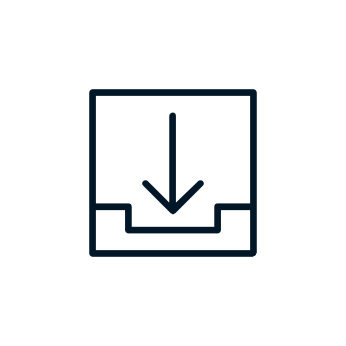
\includegraphics[height=0.5\textheight]{figures/download.png}
    \end{figure}
  \end{minipage}
\end{frame}


\section{Evaluation}

\begin{frame}<-1>[label=testing]{Testing}
  \begin{minipage}{0.49\textwidth} 
    \begin{itemize}
      \item<1-> Functionality
      \item<2-> Effectiveness
      \item<3-> Usabilty
    \end{itemize}
  \end{minipage}
  \hfill
  \begin{minipage}{0.49\textwidth} 
    \begin{figure}
      \centering
      
\includegraphics[height=0.5\textheight]{figures/test-tube.png}
    \end{figure}
  \end{minipage}
\end{frame}

\begin{frame}{Functionality}
  \begin{minipage}{0.49\textwidth}
    \begin{figure}
      \centering
      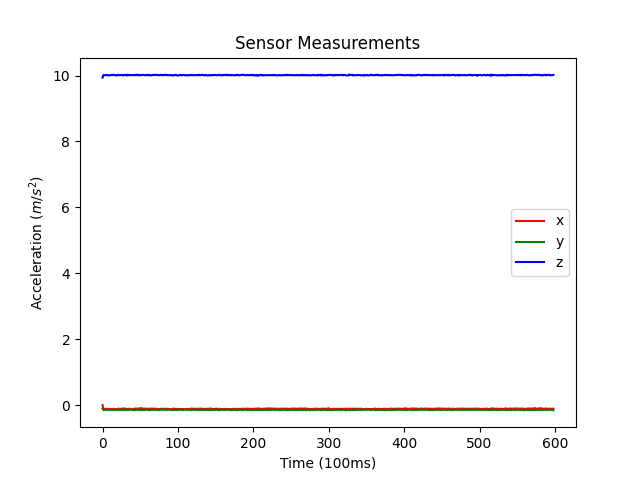
\includegraphics[height=0.45\textheight]{figures/SensorValuesBefore.png}
      \caption{recorded values before the patch}
    \end{figure}
  \end{minipage}
  \hfill
  \begin{minipage}{0.49\textwidth}
    \begin{figure}
      \centering
      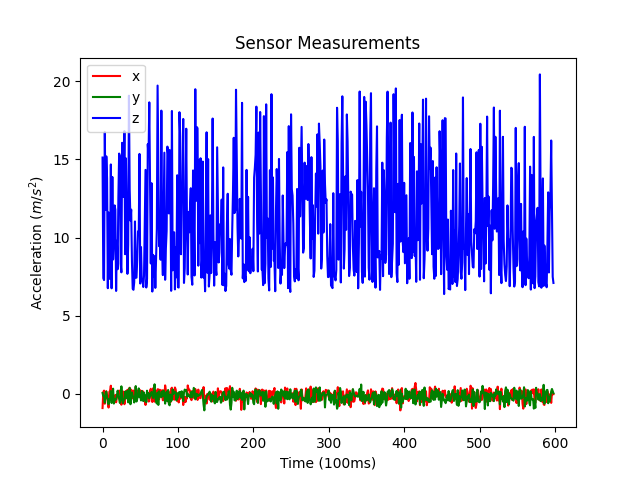
\includegraphics[height=0.45\textheight]{figures/SensorValuesAfter.png}
      \caption{recorded values after the patch}
    \end{figure}
  \end{minipage}
\end{frame}

\againframe<2>{testing}

\begin{frame}{Effectiveness}
  \begin{minipage}{0.49\textwidth}
    \begin{figure}
      \centering
      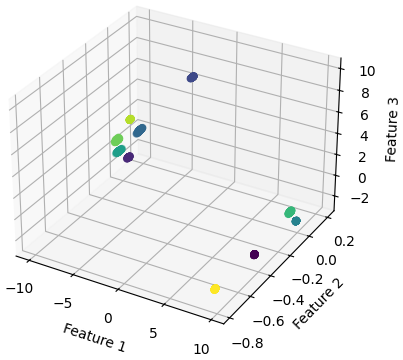
\includegraphics[height=0.45\textheight]{figures/knn_before.png}
      \caption{knn decision boundaries before the patch}
    \end{figure}
  \end{minipage}
  \hfill
  \begin{minipage}{0.49\textwidth}
    \begin{figure}
      \centering
      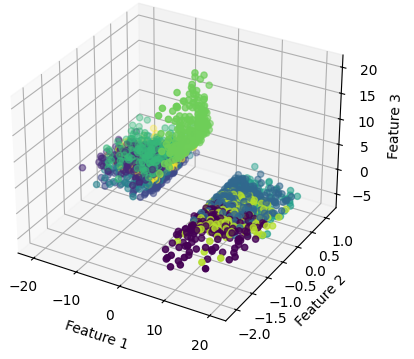
\includegraphics[height=0.45\textheight]{figures/knn_after.png}
      \caption{knn decision boundaries after the patch}
    \end{figure}
  \end{minipage}
\end{frame}

\againframe<3->{testing}

\begin{frame}{Noise Level Adjustment}
  \begin{minipage}{0.49\textwidth} 
    \begin{itemize}
      \item Increasing noise decreases fingerprintability
      \item Increasing noise decreases functionality
    \end{itemize}
  \end{minipage}
  \hfill
  \begin{minipage}{0.49\textwidth} 
    \begin{figure}
      \centering
      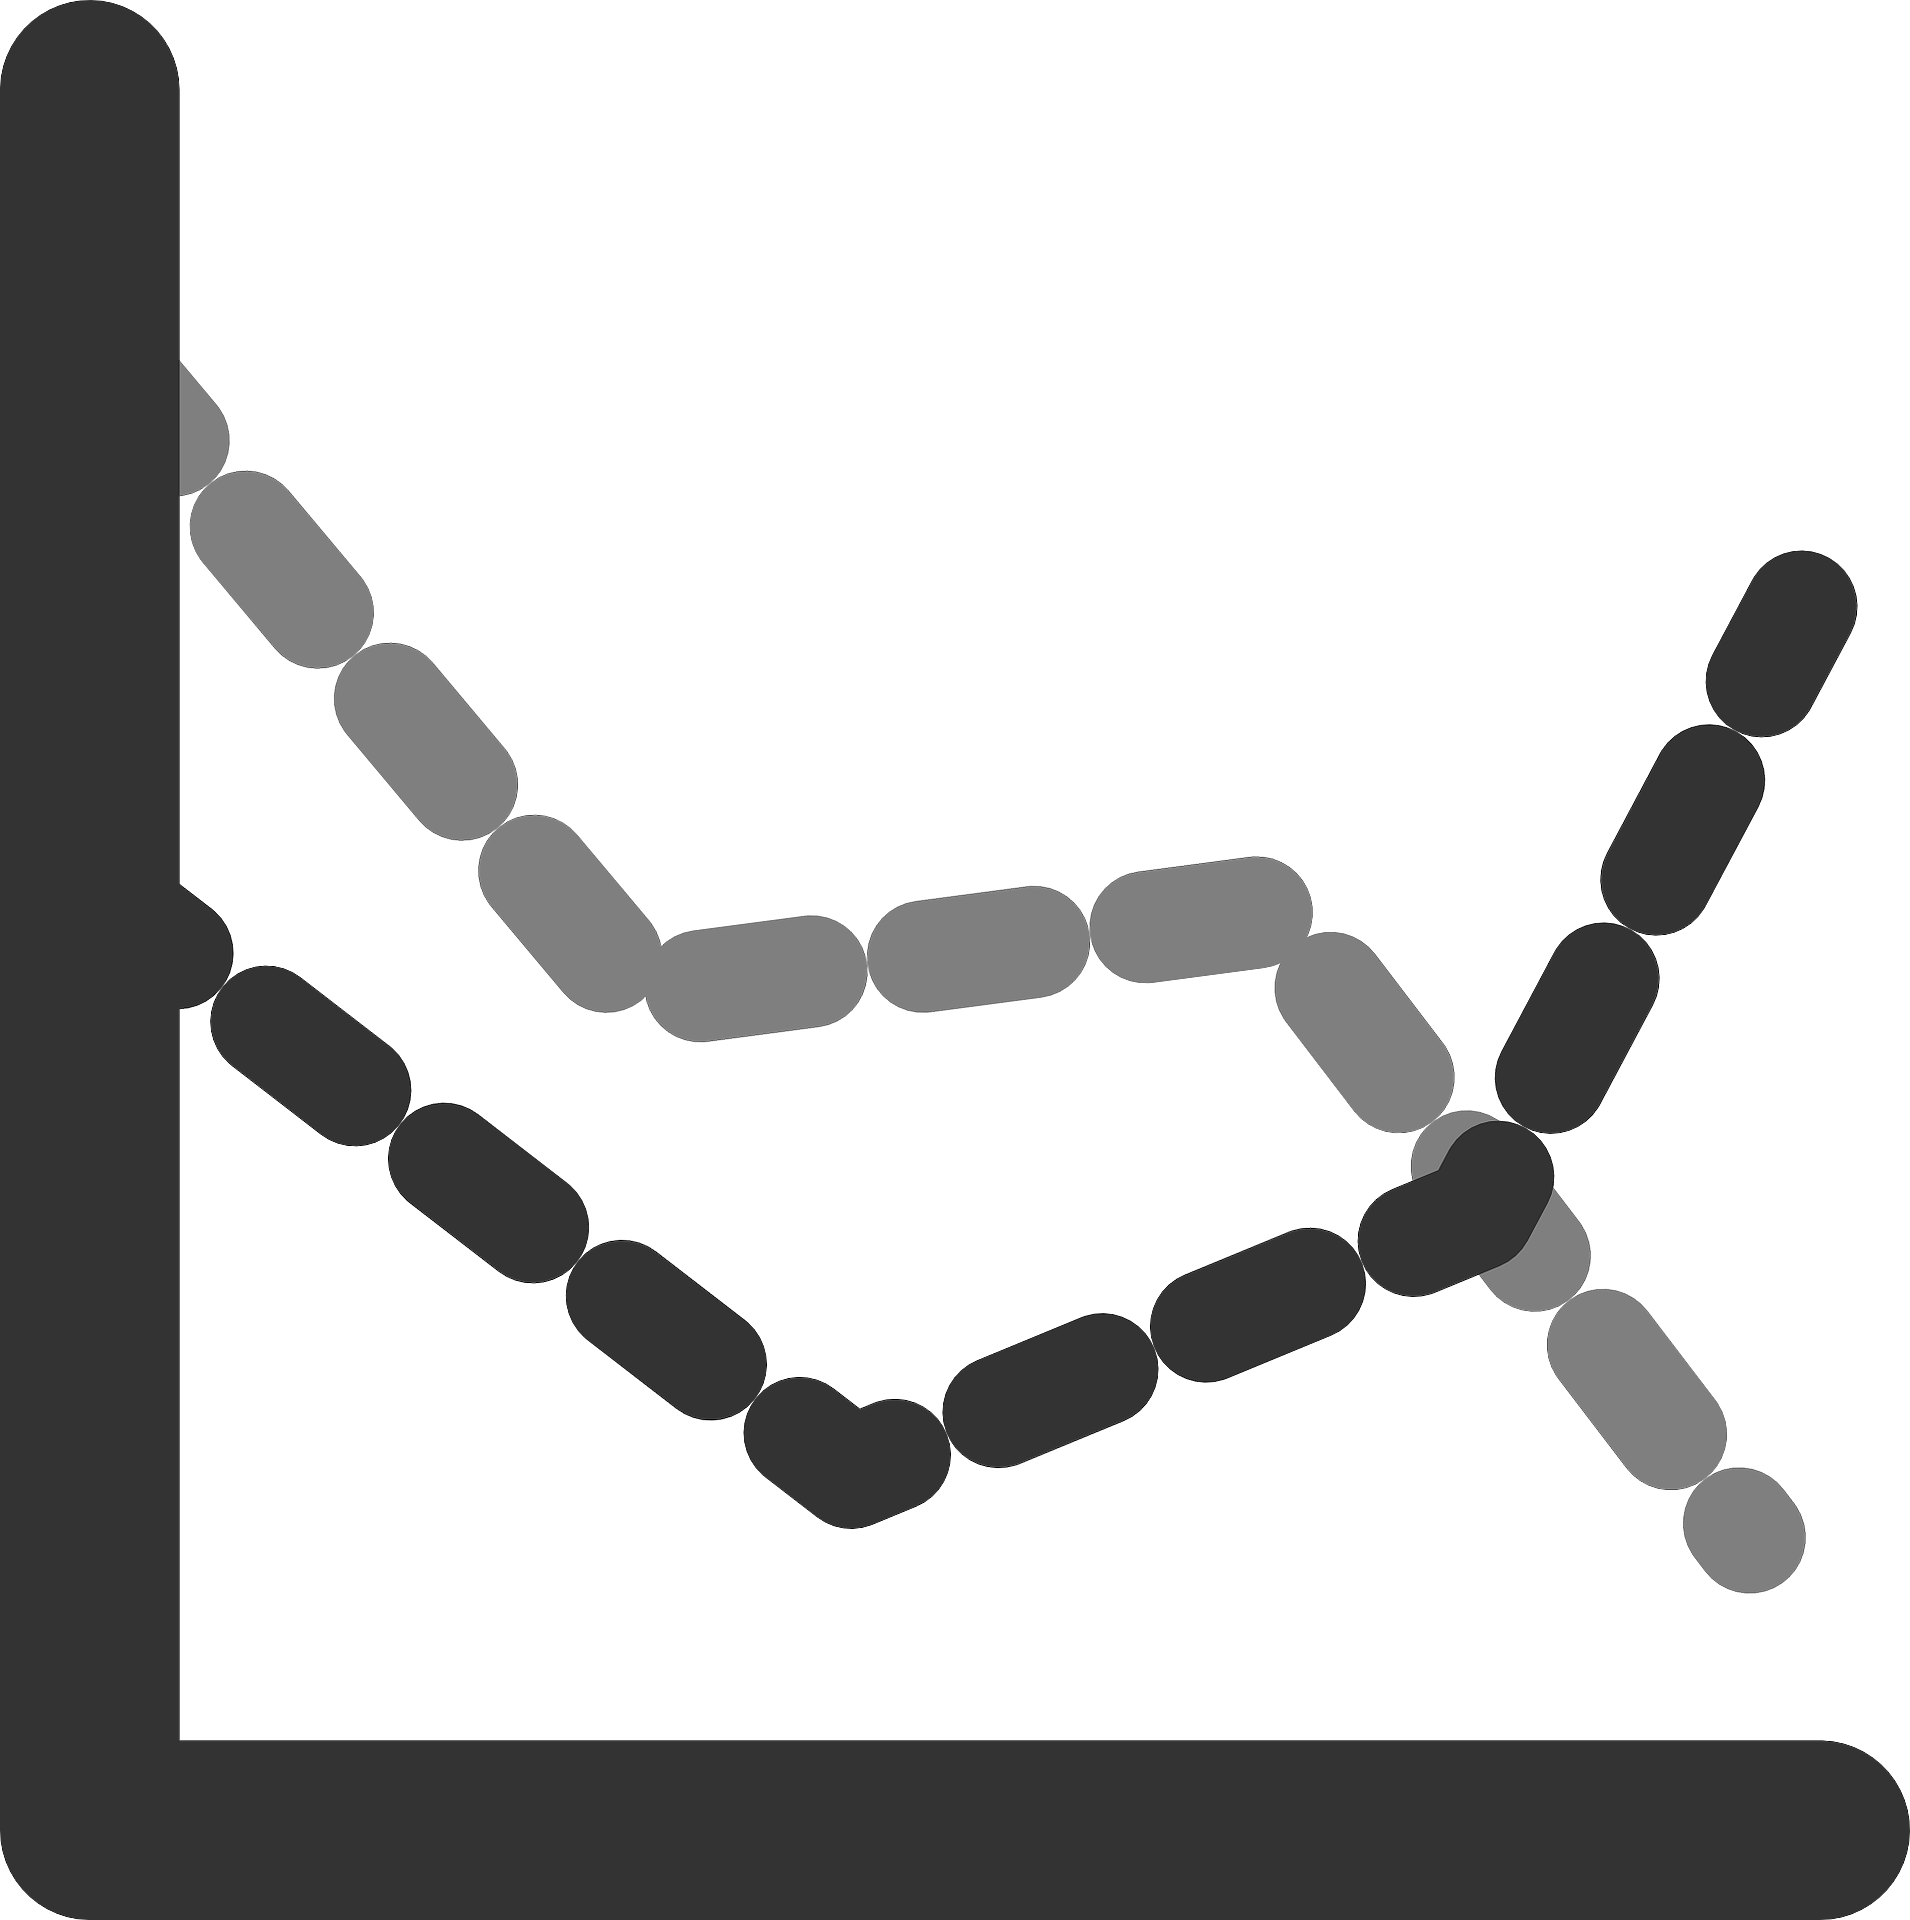
\includegraphics[height=0.5\textheight]{figures/graph.png}
    \end{figure}
  \end{minipage}
\end{frame}


\section{Discussion \& Limitations}

\begin{frame}{Discussion \& Limitations}
  \begin{minipage}{0.49\textwidth} 
    \begin{itemize}
      \item Comparing values before and after the patch
      \item Could not be done sufficiently due to limited access to supported hardware
    \end{itemize}
  \end{minipage}
  \hfill
  \begin{minipage}{0.49\textwidth} 
    \begin{figure}
      \centering
      
\includegraphics[height=0.5\textheight]{figures/comments.png}
    \end{figure}
  \end{minipage}
\end{frame}


\section*{}

\begin{frame}{Conclusion}
  \begin{minipage}{0.49\textwidth} 
    \begin{itemize}
      \item Masking the sensor values decreases fingerprintability
      \item Modifying the SensorEventListener makes it easy to incorporate the patch into the Android API
    \end{itemize}
  \end{minipage}
  \hfill
  \begin{minipage}{0.49\textwidth} 
    \begin{figure}
      \centering
      
\includegraphics[height=0.5\textheight]{figures/androguard.png}
    \end{figure}
  \end{minipage}
\end{frame}


% \begin{frame}{Bibliography}
%   ...
% \end{frame}

\end{document}
